\documentclass[border=10pt]{standalone}
\usepackage{ifthen}
\usepackage{tikz}
\usetikzlibrary[calc]

\begin{document}

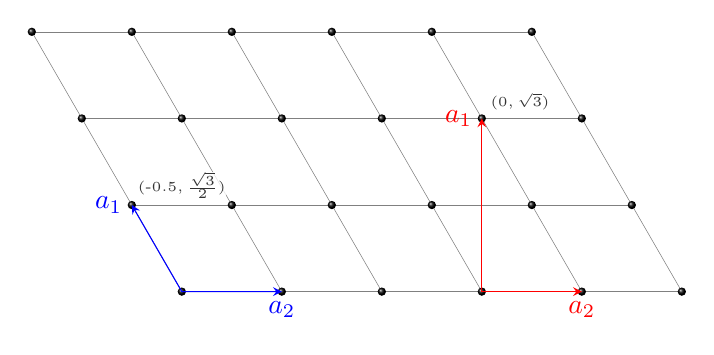
\begin{tikzpicture}
  [x=0.5in, y=0.5in]
  % define the basis vectors
  \coordinate (A1) at (1, 0);
  \coordinate (A2) at (-0.5, {sqrt(3)/2});

  % plot the lattice and grid point
  \foreach \ii in {0,...,5}{
    \foreach \jj in {0,...,3}{
      \ifthenelse{\ii=0}{
        \draw[help lines] ($ \jj *(A2) $) -- ++($ 5 *(A1) $);
      }{}
      \ifthenelse{\jj=0}{
        \draw[help lines] ($ \ii *(A1) $) -- ++($ 3 *(A2) $);
      }{}

      % Note that there is no space between the asterisk and the parenthesis: *(
      \shade[ball color=black] ($ \ii *(A1) + \jj *(A2) $) circle (1.5pt);
    }
  }

  \node[above right=2pt, fill=white, opacity=0.8, inner sep=0] at (-0.5, {sqrt(3)/2}) {\tiny $(\mbox{-}0.5, {\sqrt{3}\over 2})$};

  \draw[<->, >=stealth, blue] (-0.5, {sqrt(3)/2}) -- (0, 0)
    node[pos=0.0, left] {$a_1$}
    -- (1, 0)
    node[pos=1.0, below] {$a_2$};

  \begin{scope}
    [shift={(3, 0)}]

    \node[above right=3pt, fill=white, opacity=0.8, inner sep=0] at (0.0, {sqrt(3)}) {\tiny $(0, {\sqrt{3}})$};
    \draw[<->, >=stealth, red] (0, {sqrt(3)}) -- (0, 0)
      node[pos=0.0, left] {$a_1$}
      -- (1, 0)
      node[pos=1.0, below] {$a_2$};
  \end{scope}
\end{tikzpicture}

\end{document}
